\def\sphoyear{2011}
\setcounter{section}{0}
% Headers and Descriptions
\fancyhead[L]{\textbf{SPhO \sphoyear}} \fancyhead[R]{\textbf{Questions}}


\begin{titlepage}
\centering

{\Huge\bfseries SPhO \sphoyear}

\vspace{1cm}

{\LARGE Problem Set}

\vspace{2cm}

{\Large Compiled by: Tan Chien Hao, \texttt{www.tchlabs.net}}

\vspace{2cm}

{\Large Edited/Proofread by: Keith Chan, Sun Yu Chieh}
%Collaborators please feel free to add on!

\vspace{2cm}

{\large Suggest changes at: \github}


\vfill

{\itshape Last edited: \today}
\end{titlepage}

\begin{problem}
    A pendulum consists of a copper sphere of radius $R$ and density $\varrho$ suspended from a string. Due to the drag from the air the amplitude of the oscillation $A$ decays with time $t$ as
    \[A=A_0 \exp(-\gamma t)\]
    where $\gamma=\frac{9 \eta}{4 R^{2} \varrho}$. $A_0$ is the initial amplitude of the pendulum and $\eta$ is the viscosity of air. The measurement of the amplitudes is accurate to $1\%$ with other measurements provided below
    \sisetup{uncertainty-mode = separate}
    \begin{align*}
        &\eta=\qty{1.78\pm 0.02e-5}{\kg\per\m\per\s}\\
	    &R=\qty{5.2\pm 0.2}{\mm} \\
	    &\varrho=\qty{0.89\pm 0.05e3}{\kg\per\m\cubed}
    \end{align*}
    Evaluate the time taken for the amplitude to fall to $85\%$ of the initial amplitude $A_{0}$ and the error in this quantity. State the parameter that contributes the biggest error to the final result.
\hfill{[8]}\end{problem}

\begin{problem}
    In this question you are asked to make reasoned estimates and assumptions. These must be clearly stated.
    \begin{subproblem}
        Figure \ref{2011q2} shows an equilateral glass prism illuminated by a 100 W laser beam of wavelength $\lambda=\qty{600}{\nm}$. The refractive index of the glass of the prism is $1.50$ at $\lambda=600 \mathrm{~nm}$. The path of the light in the prism is parallel to the base of the prism. Calculate the change in weight of the prism when the beam is switched on.
        \begin{figure}[h]
	        \centering
	        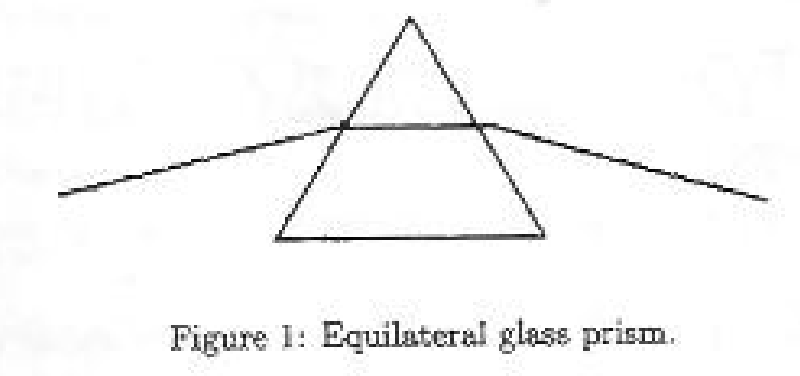
\includegraphics[width=0.8\linewidth]{spho_book_TYS_images/2011q2.png}
	        \caption{Equilateral glass prism} \label{2011q2}
        \end{figure}
    \hfill{[4]}\end{subproblem}
    
    \begin{subproblem}
        Optical tweezers, which are composed of two lasers beams, are able to manipulate small transparent spheres. Explain clearly how this can be done and why at least two beams are needed.
    \hfill{[3]}\end{subproblem}
    
    \begin{subproblem}
        Small smoke particles in air are seen under a low magnification microscope to move randomly at speed of $0.10 \mathrm{~mm}^{-1}$. The speed of sound in air is $20 \mathrm{~m} \mathrm{~s}^{-1}$. Estimate the mass of the smoke particles.
    \hfill{[3]}\end{subproblem}
\end{problem}

\begin{problem}
    Suppose that we have a string of equally spaced beads of mass m such that their surfaces are separated by a distance $d$. The beads are free to slide without friction on 4 thin wires. Suppose that there is a constant force $F$ acting on the first bead, initially at rest, and causing it to accelerate along the wire as shown in Figure \ref{2011q3}. This force acts only on the first bead and might be created by a well directed, steady stream of air. The first bead will collide with the second, which will in turn collide with the third, and so on. Suppose that all collisions are elastic.
    \begin{figure}[h]
	    \centering
	    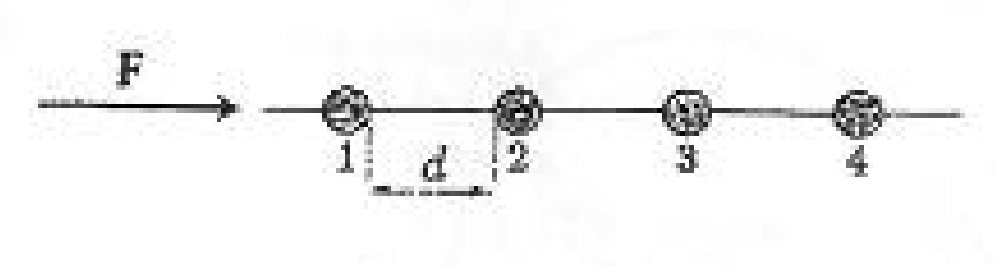
\includegraphics[width=0.7\linewidth]{spho_book_TYS_images/2011q3.png}
	    \caption{Beads on wire} \label{2011q3}
    \end{figure}
    \begin{subproblem}
        What is the speed of the first bead immediately before and immediately after its collision with the second bead?
    \hfill{[2]}\end{subproblem}

    \begin{subproblem}
        What is the speed of the second bead immediately before and immediately after its collision with the third bead?
    \hfill{[2]}\end{subproblem}

    \begin{subproblem}
        Note that the constant force is always acting upon the first bead. What is the time interval between subsequent collisions between the first and second beads? What then is the average speed of the first bead? What is the speed of the “shock wave" that travels down the wire?
    \hfill{[3]}\end{subproblem}

    \begin{subproblem}
        If the whole process is repeated, but with collisions which are perfectly inelastic, what is the terminal speed of the shock wave formed?
    \hfill{[3]}\end{subproblem}
\end{problem}

\begin{problem}
    A zoom lens system is a combination of lenses that produces a variable magnification while maintaining fixed object and image positions. The magnification is varied by moving one or more lenses along the axis. While multiple lenses are used in practice to obtain high-quality images, the effect of zooming in on an object can be demonstrated with a simple two-lens system. An object, two converging lenses, and a screen are mounted on an optical bench. The first lens, which is to the right of the object, has a focal length of $\qty{5.0}{\cm}$, and the second lens, which is to the right of the first lens, has a focal length of $\qty{10.0}{\cm}$. The screen is to the right of the second lens. Initially, an object is situated at a distance of $\qty{7.50}{\cm}$ to the left of the first lens, and the image formed on the screen has a magnification of $1.00$.
    \begin{subproblem}
        Determine the distance between the object and the screen.
    \hfill{[4]}\end{subproblem}

    \begin{subproblem}
        Both lenses are now moved along their common axis, while the object and the screen maintain fixed positions, until the image formed on the screen has - magnification of $+3.00$. Find the displacement of each lens from its initial position in (i).
    \hfill{[4]}\end{subproblem}

    \begin{subproblem}
        Can the lenses be displaced in more than one way?
    \hfill{[4]}\end{subproblem}
\end{problem}

\begin{problem}
    \begin{subproblem}
        A stick of mass density per unit length $\rho$ rests on a circle of radius $R$ (see Figure \textit{insert here}). The stick makes an angle $\theta$ with the horizontal and is tangent to the circle at its upper end. Friction exists at all points of contact, and assume that it is large enough to keep the system at rest. Find the friction force between the ground and the circle.
    \hfill{[6]}\end{subproblem}

    \begin{subproblem}
        A large number of sticks (with mass density per unit length $\rho$) and circles (with radius $R$) lean on each other, an shown in Figure \ref{2011q5}. Each stick makes an angle $\theta$ with the horizontal and is tangent to a circle at its upper end. The sticks are hinged to the ground, and every other surface is frictionless unlike in the first part of this question in (i)]. In the limit of a very large number of sticks and circles, what is the normal force between a stick and the circle it rests on very far to the right? (Assume that the last circle leans against a wall, to keep it from moving)
        \begin{figure}[h]
	        \centering
	        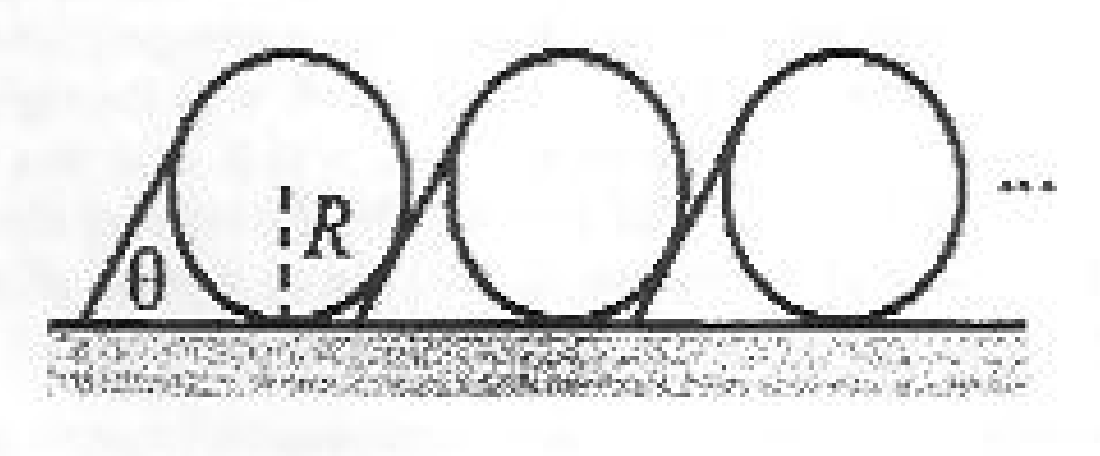
\includegraphics[width=0.7\linewidth]{spho_book_TYS_images/2011q5.png}
	        \caption{Sticks on circles}\label{2011q5}
        \end{figure}
    \hfill{[6]}\end{subproblem}
\end{problem}

\begin{problem}
    An aluminium rod $\qty{0.500}{\m}$ in length and with a cross-sectional area of $\qty{2.50}{\square\cm}$ is inserted into a thermally insulated vessel containing liquid helium at $\qty{4.20}{\K}$. The rod is initially at $\qty{300}{\K}$.
    \begin{subproblem}
        If half of the rod is inserted into the helium, how many litres of helium boil off by the time the inserted half cools to $4.20 \mathrm{~K} ?$ (Assume the upper half does not yet cool.)
    \hfill{[4]}\end{subproblem}
    \begin{subproblem}
        If the upper end of the rod is maintained at $\qty{300}{\K}$, what is the approximate boil-off rate of liquid helium after the lower half has reached $\qty{4.20}{\K}$? (Aluminium has thermal conductivity of $\qty{31.0}{\J\per\s\per\cm\per\K}$ at $\qty{4.20}{\K}$ You may ignore its temperature variation. Note that aluminium has a specific heat capacity of $\qty{902}{\J\per\kg\per\K}$ and density of $\qty{2700}{\kg\per\cubic\m}$. The density of liquid helium is $\qty{125}{\kg\per\cubic\m}$.)
    \hfill{[4]}\end{subproblem}
\end{problem}

\begin{problem}
    A soap film $(n=1.33)$ is contained within a rectangular wire frame. The frame is held vertically so that the film drains downward and forms a wedge with flat faces. The thickness of the film at the top is essentially zero. The film is viewed in reflected white light with near-normal incidence, and the first violet (the wavelength is $\qty{420}{\nm}$) interference band is observed $\qty{3.00}{\cm}$ from the top edge of the film.
    \begin{subproblem}
        Locate the first red $(\lambda=\qty{600}{\nm})$ interference band.
    \hfill{[4]}\end{subproblem}
    \begin{subproblem}
        Determine the film thickness at the positions of the violet and red bands.
    \hfill{[3]}\end{subproblem}
    \begin{subproblem}
        What is the wedge angle of the film?
    \hfill{[3]}\end{subproblem}
\end{problem}

\begin{problem}
    A solenoid of length $2 \ell$ has an inner radius $R_{1}$ and an outer radius $R_{2}$. The current through the solenoid is $I$.
    \begin{subproblem}
        Show that the magnetic flux density, $B$ at the centre of the solenoid is
        \[B=\kappa n I \ell \frac{\alpha+\left(\alpha^{2}+\beta^{2}\right)^{1 / 2}}{1+\left(1+\beta^{2}\right)^{1 / 2}}\]
        where $n$ is the number of turns per square meter and $\alpha$ and $\beta$ are functions of $R_{1}, R_{2}$ and $L$. Write down the expression for $\alpha$ and $\beta$. State the value of $\kappa$.
    \end{subproblem}
    \begin{subproblem}
        Show that the length of the wire is
        \[\ell=n V=2 \pi n\left(\alpha^{m_{1}}-1\right) \beta^{m_{1}} R_{1}^{m_{2}}\]
        where $V$ is the volume of the winding and $m_{1}, m_{2}$ and $m_{3}$ are exponents that need to be determined. State the value of $m_{1}, m_{2}$ and $m_{3}$.
    \end{subproblem}
    \begin{subproblem}
        Show that the $B$ field at the centre of the solenoid can be written as
        \[B=G\left(\frac{P \lambda \sigma}{R_{1}}\right)^{1/2}\]
        where $G$ depends on the geometry, $P$ is the dissipated power, $\lambda=\pi \pi r^{2}$ is the filling factor or fraction of the coil cross sechon oocupied by the conductor, $r$ is the radius of the wire and $\sigma$ is the conductivity.
    \hfill{[4]}\end{subproblem}
\end{problem}

\begin{problem}
    \begin{subproblem}
        A large block, with a second block sitting on top, is connected to a spring and executes horizontal simple harmonic motion as it slides across a frictionless surface with an angular frequency $\omega$. The coefficient of static friction between the two blocks is $\mu_{s}$. Derive a formula for the maximum amplitude of oscillation that the system can have if the upper block is not to slip. (Assume that the mass of the spring is negligible.)
    \hfill{[6]}\end{subproblem}
    \begin{subproblem}
        A pencil of length $L_{1}$ with the pencil point at one end and an eraser at the other end, is initially standing vertically on a table with the pencil point on the table. The pencil is let go and falls over. Derive a formula for the speed with which the eraser strikes the table, assuming that the pencil point does not move.
    \hfill{[4]}\end{subproblem}
\end{problem}


\begin{problem}
    \begin{subproblem}
        The Oscillation Project with Emulsion-tRacking Apparatus (OPERA), an experiment designed to test neutrino oscillations and exploiting the high energy muon neutrino produced at CERN Super Proton Synchrotron in Geneva and pointing towards Gran Sasso in Italy, reported that the time of flight measurements indicated that muon neutrinos travel at speed $v$ which is faster than the speed of light with $\beta=\frac{v}{c}=1+\num{1.48e-5}$, where $c$ is the speed of light in vacua. Show that it is possible for an observer moving relative to the Earth starting at CERN and moving towards Gran Sasso at some critical speed $u$ to see the muon neutrino moving backwards from Gran Sasso towards CERN and determine this critical speed.
    \end{subproblem}
    \begin{subproblem}
        A moving rod is observed to have a length of $\qty{2.00}{\m}$ and to be oriented at an angle of $\qty{30.0}{\degree}$ with respect to the direction of motion, as shown in the Figure below. The rod has a speed of $0.995\,c$.
        \begin{figure}[h]
	        \centering
	        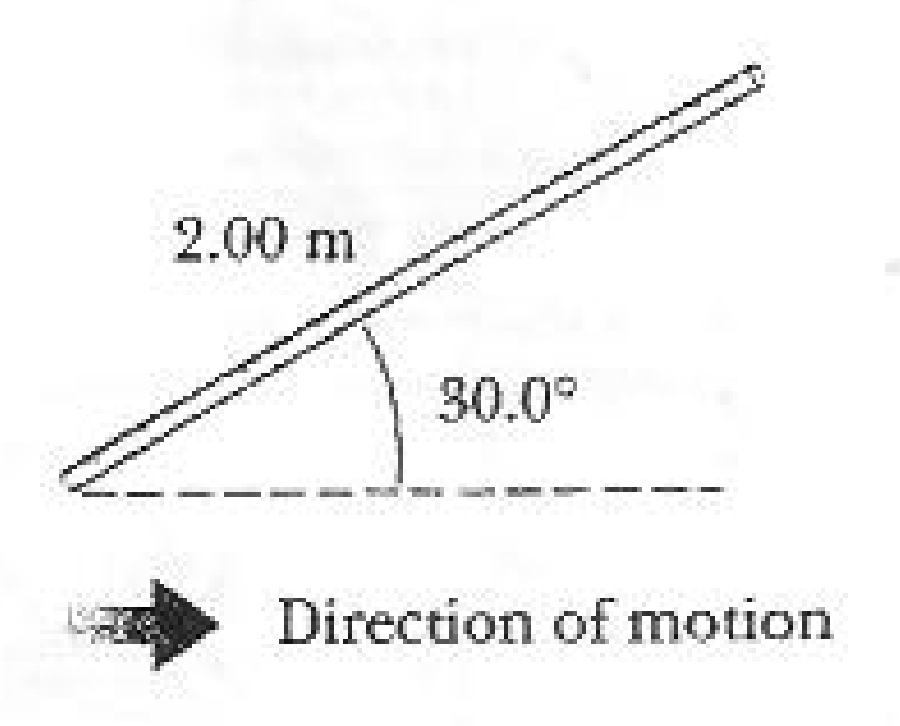
\includegraphics[width=0.7\linewidth]{spho_book_TYS_images/2011q10.png}
	          \caption{Relativistic Rod}
        \end{figure}
        \renewcommand{\theenumi}{(\alph{enumi})}
        \begin{enumerate}
            \item Determine the proper length of the rod.\hfill{[3]}
            \item What is the orientation angle in the proper frame?\hfill{[3]}
        \end{enumerate}
    \end{subproblem}
\end{problem}




